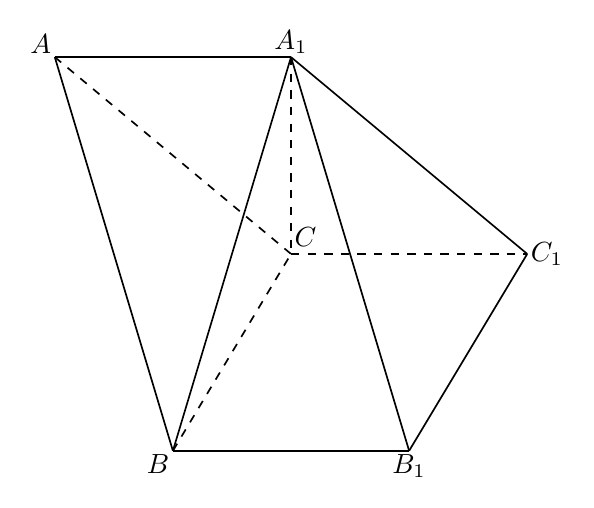
\begin{tikzpicture}[x=1cm,y=1cm,line width=.6pt]
\tikzset{lbl/.style={font=\normalsize,inner sep=1pt,fill=none}}
\coordinate (A) at (0,5);
\coordinate (A1) at (3,5);
\coordinate (B) at (1.5,0);
\coordinate (B1) at (4.5,0);
\coordinate (C) at (3,2.5);
\coordinate (C1) at (6,2.5);
% solid outline matching original
\draw (A) -- (A1);
\draw (A) -- (B);
\draw (B) -- (B1);
\draw (B) -- (A1);
\draw (A1) -- (B1);
\draw (A1) -- (C1);
\draw (B1) -- (C1);
% hidden (dashed)
\draw[dashed] (A) -- (C);
\draw[dashed] (B) -- (C);
\draw[dashed] (A1) -- (C);
\draw[dashed] (C) -- (C1);
% labels
\node[lbl,above left] at (A) {$A$};
\node[lbl,above] at (A1) {$A_{1}$};
\node[lbl,below left] at (B) {$B$};
\node[lbl,below] at (B1) {$B_{1}$};
\node[lbl,right,xshift=0.00bp,yshift=6.00bp] at (C) {$C$};
\node[lbl,right] at (C1) {$C_{1}$};
\end{tikzpicture}
